\documentclass{article}
\usepackage[T1]{fontenc}
\usepackage{lmodern}
\usepackage{graphicx}
\usepackage{amsmath,amssymb}
\usepackage[a4paper,margin=2cm]{geometry}
\usepackage[absolute,overlay]{textpos}
\setlength{\TPHorizModule}{1mm}
\setlength{\TPVertModule}{1mm}
\usepackage[indonesian]{babel}
\usepackage{hyperref}
\setlength{\emergencystretch}{2em}
% unit: Halaman 33

\begin{document}

% === Halaman 33 (llm) ===

\vspace{259.88mm}

\begin{itemize}
    \item \textit{Vig\grave{e}n\grave{e}re Cipher} menggunakan tabel Vig\grave{e}n\grave{e}re -- dinamakan Vig\grave{e}n\grave{e}re square, untuk melakukan enkripsi dan dekripsi.
    \item Setiap baris $i$ di dalam bujursangkar menyatakan huruf-huruf cipherteks yang diperoleh menggunakan \textit{Caesar Cipher} dengan kunci $k = i$.
    \item Artinya, setiap baris $i$ merupakan pergeseran huruf alfabet sejauh $i$ ke kanan
\end{itemize}

% deskripsi: Tabel Vigenere square yang menunjukkan pergeseran alfabet untuk enkripsi dan dekripsi
% bbox normalisasi: [0.4240, 0.0570, 0.9820, 0.9320]
\begin{textblock*}{117.18mm}(89.04mm,16.93mm)
\noindent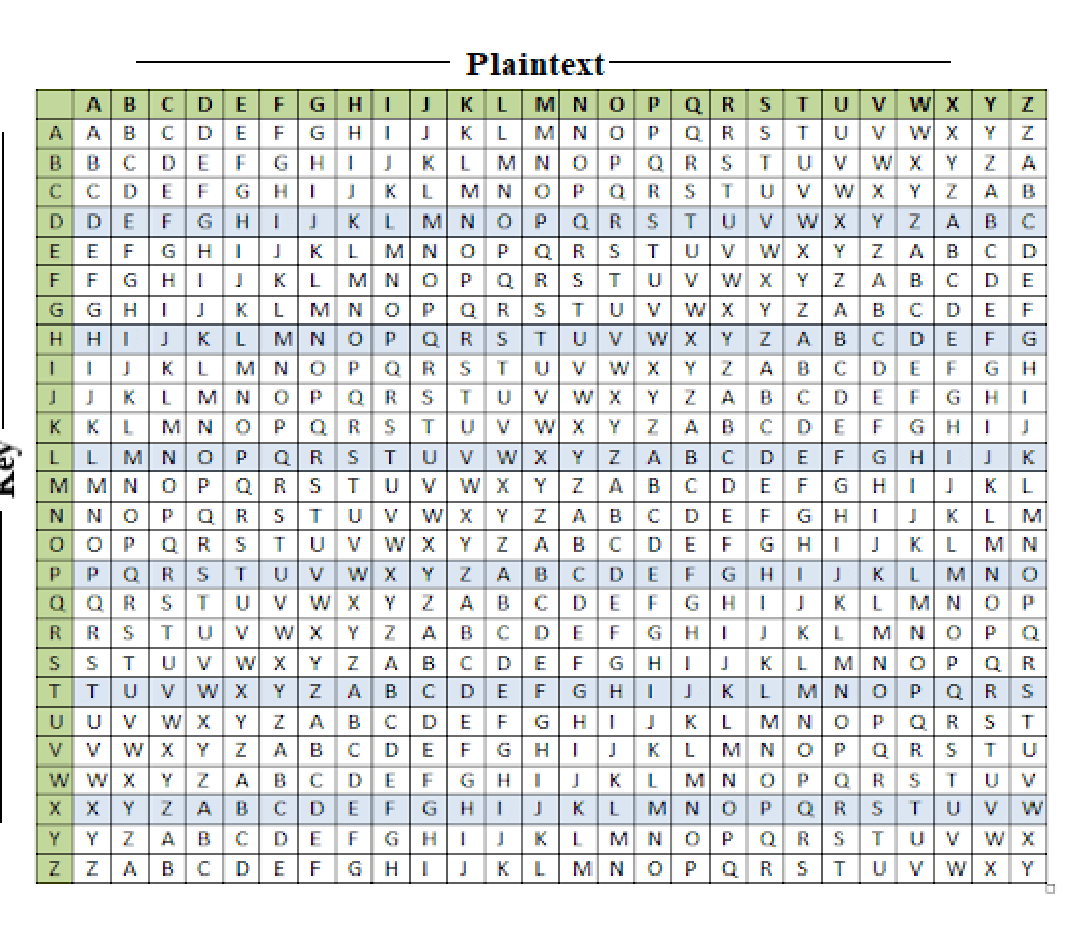
\includegraphics[width=117.18mm,height=259.88mm]{../../images/llm/page_033_img_01.png}%
\end{textblock*}

\end{document}
